% !TeX spellcheck = es_MX
\documentclass[spanish,11pt,aspectratio=1610,xcolor=table]{beamer}
% !TeX root = ../PhaseShiftNanoSensor.tex
% packages
\usepackage[spanish]{babel} \spanishdecimal{.}
\usepackage[T1]{fontenc} 
\usepackage[utf8]{inputenc}
\usepackage[scaled=0.86]{beramono}
%\usepackage{helvet}
\usefonttheme{serif}
\usepackage{animate}
		\usepackage[margin=10pt,font=scriptsize,labelfont=bf]{caption}
		\usepackage[labelformat=simple]{subcaption} 
        \usepackage{float}
		\renewcommand*{\thesubfigure}{\alph{subfigure})}
\usepackage{physics}

\usepackage{fancyhdr}
\usepackage{eurosym}
\usepackage[output-decimal-marker={,},per-mode=symbol,exponent-product={\cdot},retain-unity-mantissa=false]{siunitx}
\usepackage{csquotes}
\usepackage{tikz}
				\usepackage{tikz-3dplot}

\usepackage{textpos}
	
\usepackage{pgfplots}
\usepackage{listings}
\usepackage{mathtools}
\usepackage{textcomp}
\usepackage[version=4]{mhchem}
\usepackage{bm}
\usepackage{tabu}
\usepackage{appendixnumberbeamer}
\usepackage{bbding}
%\renewcommand{\footnotesize}{\tiny}
%\usepackage{etoolbox}
%\makeatletter    % save the meaning of \@footnotetext
%\let\BEAMER@footnotetext\@footnotetext
%\makeatother
%\usepackage{ amssymb,setspace,  graphics} 
%
%\makeatletter % restore the meaning of \@footnotetext
%\let\@footnotetext\BEAMER@footnotetext % patch the relevant command to do single spacing in footnotes
%\expandafter\patchcmd\csname beamerx@\string\beamer@framefootnotetext\endcsname
%  {\reset@font}
%  {\def\baselinestretch{\setspace@singlespace}\reset@font}
%  {}{}
%\makeatother
\makeatletter
\@newctr{footnote}[page]
\makeatother
%
\usepackage[ backend = bibtex, style = trad-abbrv,
			doi=false,isbn=false,url=false
			]{biblatex}%trad-abbrv numeric-comp
\DeclareFieldFormat[article]{volume}{\mkbibbold{#1}}
\AtEveryCitekey{\clearfield{title}}
%\DeclareBibliographyDriver{article}{\printnames{author} \newunit \printfield{year} \newunit \printfield{journaltitle} \newunit \printfield{volume} \newunit \printfield{pages} \finentry}
\addbibresource{4-References/references.bib}


% tikz libraries
\usetikzlibrary{arrows.meta}
\usetikzlibrary{calc}
\usetikzlibrary{decorations.pathreplacing}
\usetikzlibrary{positioning}
\usetikzlibrary{shapes}

% pgfplots libraries
\usepgfplotslibrary{fillbetween}

\usepackage{amsmath} % for \text
\usepackage{tikz}
\tikzset{>=latex} % for LaTeX arrow head
\usepackage{xcolor}
\colorlet{myblue}{black!40!blue}
\colorlet{myred}{black!40!red}
			\definecolor{bone}{RGB}{253,255,224}  	% bone
			\definecolor{lgreen}{RGB}{146,197,130} 	% light green,
			\definecolor{lblue}{RGB}{134,165,169}	% light blue
			\definecolor{lgray}{RGB}{118,118,118}	% light gray
			\definecolor{dgreen}{RGB}{83,111,80}	% dark green

\usepackage{appendixnumberbeamer}
		
\usepackage{multicol}						% for pages with multiple text columns, e.g. References
	\setlength{\columnsep}{20pt} 				% space between columns; default 10pt quite narrow
\usepackage{multirow}

% !TeX root = ../PhaseShiftNanoSensor.tex
% colors
% tum main colors
\definecolor{tumblue}{RGB}{0, 101, 189}
\definecolor{tumblack}{RGB}{0, 0, 0}
\definecolor{tumwhite}{RGB}{255, 255, 255}

% tum blue tones (shades !85, !70, !55 allowed)
\definecolor{tumdarkerblue}{RGB}{0, 51, 89}
\definecolor{tumdarkblue}{RGB}{0, 82, 147}
\definecolor{tummidblue}{RGB}{0, 115, 207}
\definecolor{tumlightblue}{RGB}{100, 160, 200}
\definecolor{tumlighterblue}{RGB}{152, 198, 234}

% tum grey tones
\definecolor{tumdarkergrey}{RGB}{44, 44, 45}
\definecolor{tumdarkgrey}{RGB}{88, 88, 90}
\definecolor{tumgrey}{RGB}{156, 157, 159}
\definecolor{tumlightgrey}{RGB}{217, 218, 219}
\definecolor{tumlightergrey}{RGB}{235, 236, 237}

% tum accent colors (shades !85, !70, !55 allowed)
\definecolor{tumorange}{RGB}{227,114,34}
\definecolor{tumgreen}{RGB}{162,173,0}
\definecolor{tumivory}{RGB}{218,215,203}

% tum extended palette (shades !85, !70, !55 allowed)
\definecolor{tumviolet}{RGB}{105,8,90}
\definecolor{tumdarkviolet}{RGB}{15,27,95}
\definecolor{tumturquois}{RGB}{0,119,138}
\definecolor{tumdarkgreen}{RGB}{0,124,48}
\definecolor{tummidgreen}{RGB}{103,154,29}
\definecolor{tumbrightyellow}{RGB}{255,220,0}
\definecolor{tumbrightorange}{RGB}{249,186,0}
\definecolor{tumbrightred}{RGB}{214,76,19}
\definecolor{tumred}{RGB}{196,7,27}
\definecolor{tumdarkred}{RGB}{156,13,22}


% tum presentation colors (styleguide, p.266)
\definecolor{tumpyellow}{RGB}{255,180,0}
\definecolor{tumporange}{RGB}{255,128,0}
\definecolor{tumpred}{RGB}{229,52,24}
\definecolor{tumpdarkred}{RGB}{202,33,63}
\definecolor{tumpblue}{RGB}{0,153,255}
\definecolor{tumpbrightblue}{RGB}{65,190,255}
\definecolor{tumpgreen}{RGB}{145,172,107}
\definecolor{tumpbrightgreen}{RGB}{181,202,130}

% custom thesis colors
\definecolor{biomass}{RGB}{0, 122, 55}
\definecolor{co2}{RGB}{160, 160, 160}
\definecolor{coal}{RGB}{100, 100, 100}
\definecolor{cool}{RGB}{0, 0, 255}
\definecolor{demand}{RGB}{25, 25, 25}
\definecolor{diesel}{RGB}{116, 66, 65}
\definecolor{gas}{RGB}{128, 64, 0}
\definecolor{elec}{RGB}{255, 170, 0}
\definecolor{heat}{RGB}{230, 112, 36}
\definecolor{hydro}{RGB}{198, 188, 240}
\definecolor{hydrogen}{RGB}{198, 188, 240}
\definecolor{imp}{RGB}{128, 128, 200}
\definecolor{lignite}{RGB}{116, 66, 65}
\definecolor{nuclear}{RGB}{192, 34, 16}
\definecolor{oil}{RGB}{116, 66, 65}
\definecolor{overproduction}{RGB}{190, 0, 99}
\definecolor{slack}{RGB}{163, 74, 130}
\definecolor{solar}{RGB}{243, 174, 0}
\definecolor{storage}{RGB}{60, 36, 154}
\definecolor{wind}{RGB}{122, 179, 225}
\definecolor{stock}{RGB}{222, 222, 222}

% custom building type colors
\definecolor{basin}{RGB}{110, 75, 56}
\definecolor{chapel}{RGB}{177, 121, 91}
\definecolor{church}{RGB}{177, 121, 91}
\definecolor{commercial}{RGB}{129, 162, 190}
\definecolor{farm}{RGB}{202, 178, 214}
%\definecolor{garage}{RGB}{253, 191, 111}
\definecolor{greenhouse}{RGB}{255, 127, 0}
%\definecolor{hospital}{RGB}{129, 221, 190}
\colorlet{hospital}{tumturquois}
%\definecolor{hotel}{RGB}{227, 26, 28}
\colorlet{hotel}{tumorange!50}
\definecolor{house}{RGB}{181, 189, 104}
\definecolor{industrial}{RGB}{240, 198, 116}
\definecolor{office}{RGB}{129, 162, 190}
%\definecolor{public}{RGB}{129, 162, 190}
\definecolor{residential}{RGB}{181, 189, 104}
\definecolor{restaurant}{RGB}{227, 26, 28}
%\definecolor{retail}{RGB}{129, 162, 190}
\definecolor{school}{RGB}{29, 103, 214}
%\definecolor{warehouse}{RGB}{98, 134, 6}
\colorlet{warehouse}{tumgrey!50}
\colorlet{garage}{tumgrey!75}
\colorlet{public}{commercial!50}
\colorlet{other}{tumgrey}
\colorlet{retail}{commercial!75}

% !TeX root = ../PhaseShiftNanoSensor.tex
% Pgfplots settings and styles
\pgfplotsset{%
    compat=1.12,
    major grid style={thin, color=gray!25},
    minor grid style={thin, color=gray!25},
    tumaxisstyle/.style={
        axis line style={opacity=0}, major tick style={draw=none},
        ymajorgrids, xmajorgrids},
        every axis/.append style={font=\footnotesize},
        legend style={draw=none, legend cell align=left},
    /pgfplots/square ybar legend/.style={
        /pgfplots/legend image code/.code={%
            \fill[##1,/tikz/.cd,bar width=.5em]
            plot coordinates { (\pgfplotbarwidth,.5em)};}}
}

% Tikz styles
\tikzset{%
    flowbox/.style={rectangle split, rectangle split parts=2, 
                    rectangle split part fill={jddarkblue,jddarkblue!20},
                    align=center},
    conn/.style={draw=jdblue, -{Latex[length=3mm]}, 
                 rounded corners=3pt},
    hidden/.style={-{Latex[length=2mm]}, draw=tumdarkgrey,
                   rounded corners=2pt, densely dotted},
    concept/.style={fill=jddarkgrey!15},
    darrows/.style={{Latex[length=2mm]}-{Latex[length=2mm]}},
    onslide/.code args={<#1>#2}{\only<#1>{\pgfkeysalso{#2}}},
    fb-muted/.style={rectangle split part fill={jdgrey,jdgrey!15}},
    fb-highlight/.style={rectangle split part fill={jdgreen,jdgreen!20}}
}

% Tikz commands
\newcommand{\fbtitle}[1]{\textbf{\textcolor{jdwhite}{#1}}}

% beamer dimensions
\newlength{\maxheight}
\setlength{\maxheight}{\textheight}
\addtolength{\maxheight}{-\headheight}
\addtolength{\maxheight}{-\footheight}
\addtolength{\maxheight}{-2em} % guessing :-(

\AtBeginDocument{%
\newlength{\squeezetwo}
\setlength{\squeezetwo}{.495\paperwidth}
%
\newlength{\squeezethree}
\setlength{\squeezethree}{.33\paperwidth}
%
\newlength{\loosethree}
\setlength{\loosethree}{.29\textwidth}
}

% listings settings
\lstset{
    basicstyle={\color{jddarkgrey}\ttfamily},
    identifierstyle=\color{jddarkblue},
    commentstyle={\color{jdgreen}},
    stringstyle={\color{gred}},
    keywordstyle={\color{jddarkerblue}},
    emphstyle={\color{jdlightblue}},
    emph={urbs,rivus},
    texcl=true
}

% hyperref settings
\hypersetup{colorlinks=true,linkcolor=,urlcolor=jdgreen}


\usetheme{JD}
\beamertemplatenavigationsymbolsempty

%\svgpath{{1-Theory/figs},{5-Apendices/figs},{2-Results/figs}}
\graphicspath{{5-Apendices/figs},{0-5-Introduccion/figs}}

\title
    [AuNPs parcialmente embebidas]
    {\textit{Optical properties of partially embedded nanospheres}}

\subtitle{Examen de maestría: Propiedades ópticas de nanoesferas parcialmente embebidas} % short version unused by this template
\author
    [J. Urrutia]
    {Jonathan A. Urrutia Anguiano$^1$}
\institute
    [PCF OyF]
    {Facultad de Ciencias, UNAM\\
 	Dr. Alejandro Reyes Coronado$^1$\\[2em]
    $^1$Departamento de Física,\\
    Facultad de Ciencias, UNAM
    }
\date
    []
    {}

\titlegraphic{%
\begin{picture}(0,0)
    \put(0,-150){\makebox(0,0)[rt]{
\includegraphics[scale=.45]{Latex/setup/pcf-logo.png}}}
  \end{picture}
  }

\begin{document}

\maketitle

% !TeX root = ../presentation.tex

\section*{Introducción}
%----------------------------------------------------------------------------------
\begin{frame}{{Antecedentes}}

    \begin{alertblock}{Metasuperficies plasmónicas para biosensado}
        \begin{itemize}%[<+->]
         \itemsep9pt
         \item Arreglos bidimensionales de \textbf{nanoestructuras metálicas} (meta-átomos) soportadas por un sustrato.$^1$
        \end{itemize}
    \end{alertblock}
    
    \begin{center}
  	\begin{tikzpicture}[node distance=1em and 1em,font=\small]
        \path (0,0) node [flowbox] (bio) {\fbtitle{Meta-átomos}\vphantom{yÖ}
	    \nodepart{two}
         \begin{minipage}{.25\textwidth} \begin{itemize}
			\item Geometría
			\item Material
			\item Distribución
               \begin{itemize}
                  \item Desordenada $^{4,5}$
                  \item Periódica $^{2,3}$
               \end{itemize}
            \item \textbf{Perfecto soporte sobre sustrato}
         \end{itemize}\end{minipage}
        };

        \node[flowbox, below = of bio] (exp) {\fbtitle{Respuesta óptica}\vphantom{yÖ}
        \nodepart{two}
         \begin{minipage}{.25\textwidth} \begin{itemize}
            \item Resultados experimentales$^{2,3,4,5}$
            \item Simulaciones numéricas$^{2,3,4}$
            \item Teorías de medio efectivo$^5$
         \end{itemize}\end{minipage}
        };

        \node at (7,-1){\includegraphics[scale = .6]{background.png}};

        \node[draw,circle,inner sep=0.5pt, font=\tiny] at (2.85, 1) {A};
%         \node at (2.85, 1) {\ding{173}}; %2

        \node[draw,circle,inner sep=0.5pt, font=\tiny] at (5.8,1.2) {B};
%         \node at (5.8,1.2) {\ding{174}};   %3

        \node[draw,circle,inner sep=0.5pt, font=\tiny] at (6,-1.5) {C};
%         \node at (6,-1.5) {\ding{175}}; %4

        \node[draw,circle,inner sep=0.5pt, font=\tiny] at (9.6,1) {D};
%         \node at (9.6,1) {\ding{176}}; %5
    \end{tikzpicture}
    \end{center}   
    
    \vspace*{-4em}
    \begin{columns}
        \column{.35\textwidth}
        \column{.65\textwidth}
        \noindent\rule{.25\textwidth}{0.4pt}	
         \begin{spacing}{0}\fontsize{4}{5} \selectfont
            $^1$ \fullcite{gonzalez-alcalde_large_2020}\\
            $^{2\text{, A}}$ \fullcite{feuz_improving_2010}\\
            $^{3\text{, B}}$ \fullcite{kabashin_plasmonic_2009}\\
            $^{4\text{, C}}$ \fullcite{qiu_dual_2020}\\
            $^{5\text{, D}}$ \fullcite{svedendahl_refractometric_2014}
         \end{spacing}	
   \end{columns}
\end{frame}

% %----------------------------------------------------------------------------------
% \begin{frame}{{Objetivo}}
% \begin{columns}
%    \column{.55\textwidth}
%    \begin{alertblock}{Incrustamiento parcial de meta-átomos en el sustrato}
%         \begin{itemize}%[<+->]
%          \item Resultados del proceso de fabricación$^1$
%          \item Característica deseable para metasupeficies enfocadas para biosensado (Acoplamiento con sistemas de microfluídica)
%          \item ¿Cuál es su efecto en la respuesta óptica?
%         \end{itemize}
%     \end{alertblock}
%    \column{.45\textwidth}
%
%    \begin{center}
%   	\begin{tikzpicture}[node distance=1em and 1em,font=\small]
%         \path (0,0) node [flowbox] (bio) {\fbtitle{Sistema de estudio}\vphantom{yÖ}
% 	    \nodepart{two}
%          \begin{minipage}{.95\textwidth}
%          Nanopartíula esférica apta para biosensado en metasuperficies\\
%
%          \begin{itemize}
% 			\item Meta-átomo: 12.5 nm AuNP
% 			\item Matriz: Aire
% 			\item Sustrato: Vidrio
%          \end{itemize}\end{minipage}
%         };
%     \end{tikzpicture}
%     \end{center}
% \end{columns}
%
%     \begin{center}
%   	\begin{tikzpicture}[node distance=1em and 1em,font=\small]
%         \node at (0,0) {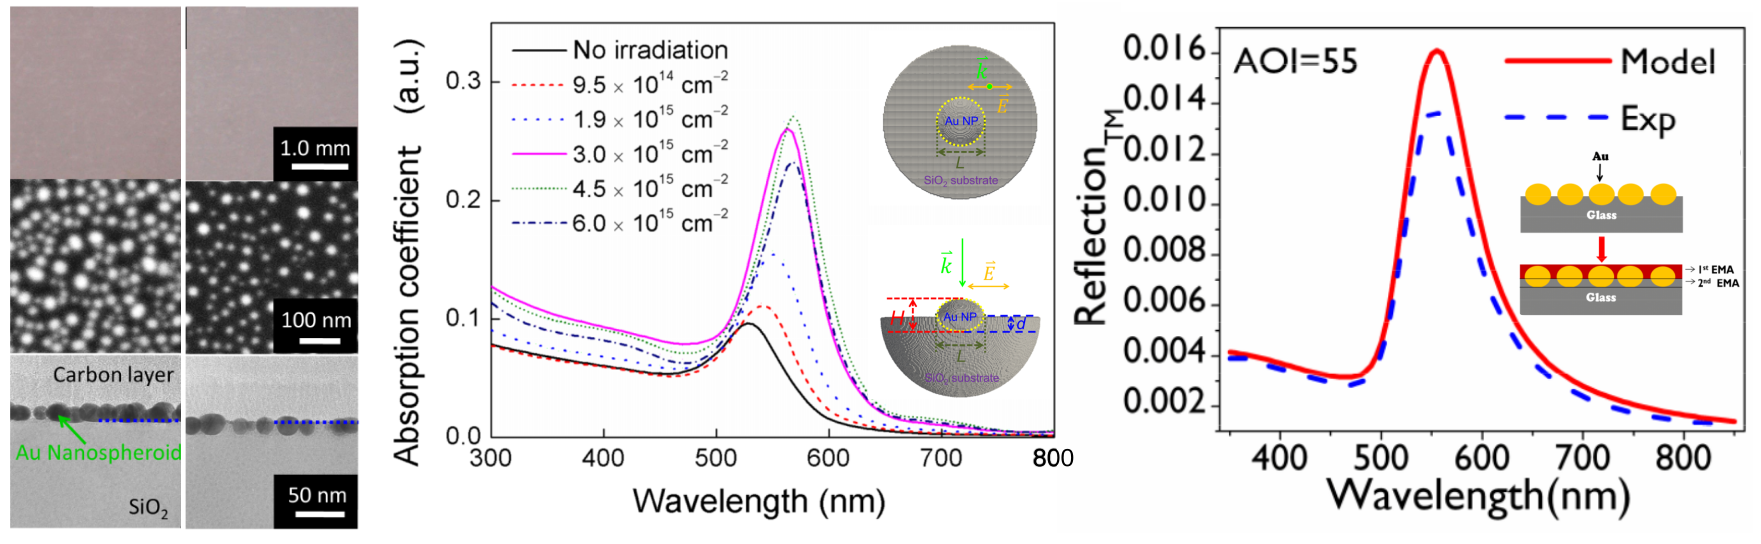
\includegraphics[scale = .7]{embedding.png}};
%
%         \node at (-5.35,1.45) {\ding{172}}; %1
%         \node at (1.25,1.35) {\ding{173}};   %2
%     \end{tikzpicture}
%     \end{center}
%
%     \vspace*{0em}
%         \noindent\rule{.25\textwidth}{0.4pt}
%          \begin{spacing}{0}\fontsize{4}{12} \selectfont
%             $^1$ \fullcite{meng_anisotropic_2015}\\
%             $^2$ \fullcite{moirangthem_enhanced_2012}
%          \end{spacing}
% \end{frame}


%----------------------------------------------------------------------------------
\begin{frame}{Objetivo}{Estudio del incrustamiento parcial de meta-átomos en el sustrato}
   \begin{center}
  	\begin{tikzpicture}[node distance=1em and 1em,font=\small]
        \path (-7.5,0) node [flowbox] (bio) {\fbtitle{Incrustamiento de meta-átomos}\vphantom{yÖ}
	    \nodepart{two}
         \begin{minipage}{.3\textwidth}
         \begin{itemize}%[<+->]
         \item Proceso de fabricación$^1$
         \item Característica deseable para biosensado
            \begin{itemize}
            \item Acoplamiento con  sistemas de microfluídica
            \end{itemize}
         \item \textbf{¿Detección óptica?}
        \end{itemize}\end{minipage}
        };
%
         \node at (0,-1.5) {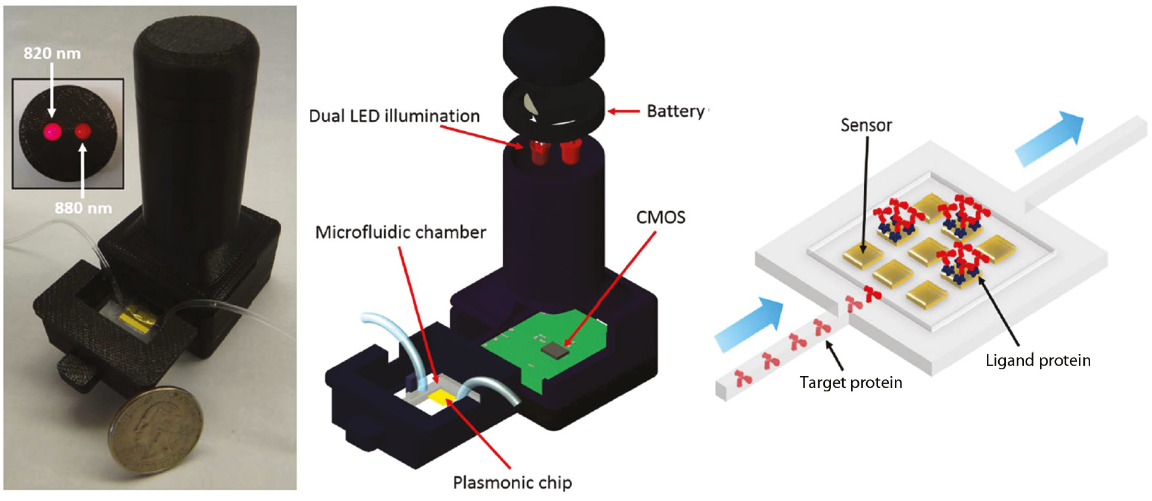
\includegraphics[scale = .3, trim = {0 0 0 0}, clip]{micro.png}};

         \node at (0,+1.5) {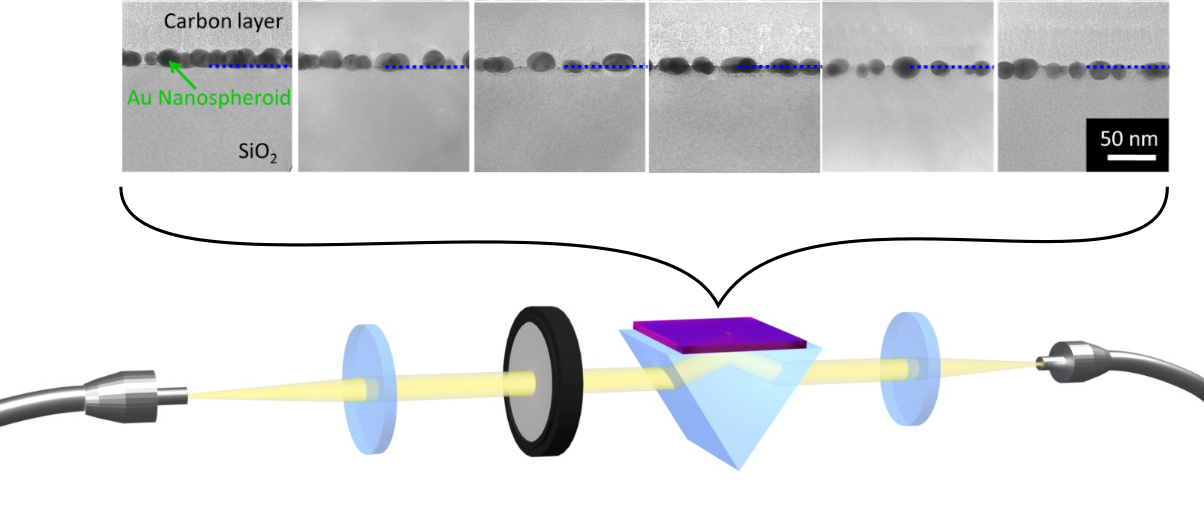
\includegraphics[scale = 1.05, trim = {30 80 10 0}, clip]{exp-NPs.png}};
    \end{tikzpicture}
\end{center}

    \vspace*{0em}
        \noindent\rule{.25\textwidth}{0.4pt}
         \begin{spacing}{0}\fontsize{4}{12} \selectfont
            $^1$ \fullcite{meng_anisotropic_2015}\\
            $^2$ \fullcite{moirangthem_enhanced_2012}
         \end{spacing}
\end{frame}


%----------------------------------------------------------------------------------
\begin{frame}{Sistema de interés}{Meta-átomo: Nanopartíula (NP) esférica de oro (Au) apta para biosensado}

      \begin{center}
  	\begin{tikzpicture}[node distance=1em and 1em,font=\small]
        \path (-7.5,-1) node [flowbox] (bio) {\fbtitle{FC-UNAM$^1$ -- INAOE$^{2}$}\vphantom{yÖ}
	    \nodepart{two}
         \begin{minipage}{.35\textwidth}
          Desarrollo de un biosensor plasmónico:\\

          \begin{itemize}
            \item Colaboración teórico-experimental
			\item Metasuperficie desordenada
            \item Mediciones de reflectancia
%                \begin{itemize}
%                   \item Polarización $s$
%                   \item Polarización $p$
%                \end{itemize}
% 			\item Incidencia oblicua
         \end{itemize}\end{minipage}
        };

        \node at (-2.25,-0.25) {Esquema del sistema experimental$^3$:};
          \node at (0,-1.75) {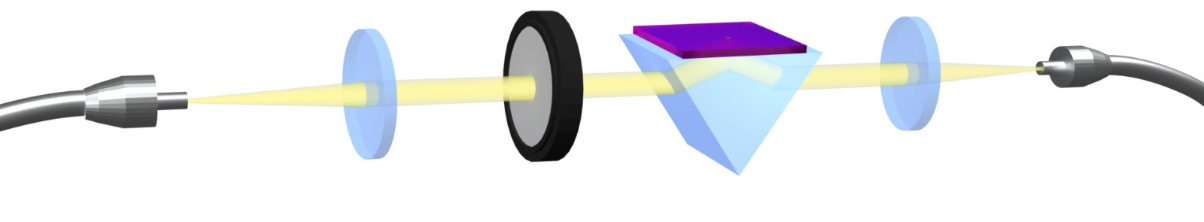
\includegraphics[scale = .8]{sistExp.png}};

        \node at (-3,-0.75) {\footnotesize Fuente de luz blanca};
        \node at (1.,-0.75) {\footnotesize Muestra sobre prisma};
        \node at (3.5,-0.75) {\footnotesize Detector};

        \node at (-1.6,-2.5) {\footnotesize Lente};
        \node at (-.25,-2.5) {\footnotesize Polarizador};
        \node at (2.1,-2.5) {\footnotesize Lente};

        \path (-7.5,-4) node [flowbox] (bio) {\fbtitle{Meta-átomo:}\vphantom{yÖ}
	    \nodepart{two}
         \begin{minipage}{.25\textwidth}
          \begin{itemize}
			\item AuNP esférica
            \item Radio $a$: 12.5 nm
			\item Matriz: Aire
			\item Sustrato: Vidrio
			\item Incrustamiento parcial
         \end{itemize}\end{minipage}
        };

        \node at (0,-4.75) {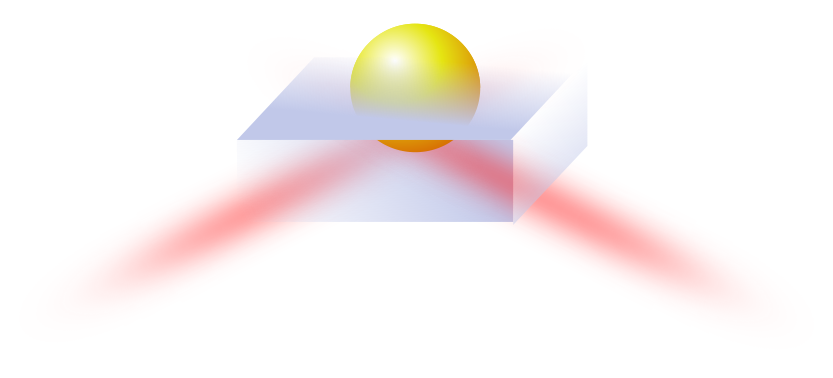
\includegraphics[scale = 1.1]{NP.png}};
        \node at (-3,-3.0) {Esquema del meta-átomo:};

        \node at (1,-3.5) {\footnotesize Matriz};
        \node at (.5,-4.75) {\footnotesize Sustrato};

    \end{tikzpicture}
    \end{center}

    \vspace*{-3.5em}
        \noindent\rule{.25\textwidth}{0.4pt}
         \begin{spacing}{0}\fontsize{4}{12} \selectfont
            $^1$ Grupo de Nanoplasmónica\\
            $^2$ Grupo de Biofotónica y Grupo de Optoelectrónica de semiconductores orgánicos e híbridos\\
            $^3$ Esquema realizado Juan Pablo Cuanalo Fernández.
         \end{spacing}
\end{frame}





\end{document}
